14. $y=\cfrac{2x^2+5x+2}{x+2}\cdot(x-1)=\cfrac{(2x+1)(x+2)}{x+2}\cdot(x-1)=2x^2-x-1,\ x
eq-2.$ Построим параболу по трём точкам $(1;0),\ \left(-\cfrac{1}{2};0
ight),\ \left(\cfrac{1}{4};-\cfrac{9}{8}
ight).$
$$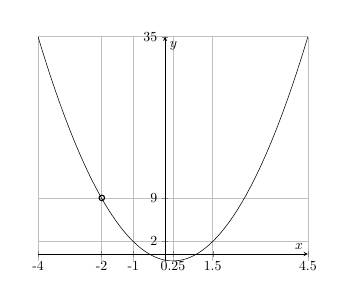
\begin{tikzpicture}[scale=0.5]
\begin{axis}[
    axis lines = middle,
    grid=major,
    legend pos={south west},
    xlabel = {$x$},
    ylabel = {$y$},
    %ymin=-80,
    %ymax=250,
    xtick={-4, -2, -1, 0.25, 1.5, 4.5},
    xticklabels={-4, -2, -1, 0.25, 1.5, 4.5},
    ytick={35,9,2},
    yticklabels={35,9,2}             ]
	\addplot[domain=-4:4.5, samples=100, color=black] {(2*x+1)*(x-1)};
%\addplot[domain=-3.1:2.5, samples=100, color=red] {70*abs(1-2*abs(abs(x)-2))-10*x^2+10*x-70};
	%\addlegendentry{$\text{Рис. 1}$};
\end{axis}
\draw (1.62,1.6) circle (2pt);
\end{tikzpicture}$$
